\chapter{Milieux continus et élasticité}\label{ch:b3:continuum-elasticity}

Collez l'oreille à un long rail d'acier pendant qu'un ouvrier le frappe
au loin~: vous entendez deux chocs --- l'un par l'acier, l'autre par
l'air, séparés d'une seconde ou plus. La roche, l'acier, l'os et le
caoutchouc transmettent tous forces et ondes comme un fluide transmet
la pression, mais avec quelque chose qu'aucun fluide n'a~: ils
résistent aux \emph{changements de forme}, et pas seulement aux
changements de volume. Le volume de deuxième année a bâti la mécanique
des fluides sur deux idées, la particule de matière et le champ de
pression~; ce chapitre les étend aux solides. Le déplacement de chaque
particule devient un champ, sa distorsion locale une \emph{déformation},
les forces intérieures une \emph{contrainte}, et entre les deux se
tient la carte d'identité du solide, la \omterm{thm:b3:continuum-elasticity:hooke}{loi de Hooke} avec ses deux
constantes élastiques. Le gain va du quotidien --- pourquoi les câbles
s'allongent, pourquoi les bouteilles éclatent, comment un plongeoir
fléchit --- au planétaire~: les séismes envoient à travers la Terre
exactement les deux \omterm{prop:b3:continuum-elasticity:waves}{ondes élastiques} que ce chapitre prédit, et leurs
temps d'arrivée furent la première auscultation de l'intérieur de notre
planète.

\section{La déformation~: décrire la distorsion}

\begin{definition}[Champ de déplacement et tenseur des déformations]\label{def:b3:continuum-elasticity:strain}
\index{champ de déplacement}\index{tenseur des déformations}\index{dilatation}
Quand un solide se déforme, la particule initialement en $\vect r$ va
en $\vect r + \vect u(\vect r)$~: $\vect u$ est le \emph{champ de
déplacement}. Pour de petites déformations, la distorsion locale est
mesurée par le \emph{tenseur des déformations}, le tableau symétrique
\[
\varepsilon_{ij} = \frac12\Big(
 \frac{\partial u_i}{\partial x_j} + \frac{\partial u_j}{\partial x_i}
\Big) , \qquad i, j \in \{x, y, z\} .
\]
Une composante diagonale $\varepsilon_{xx}$ est l'allongement relatif
du matériau selon $x$ (sans dimension, par exemple $\num{e-3}$ pour un
câble d'acier en service)~; une composante hors diagonale
$\varepsilon_{xy}$ est la moitié de la fermeture de l'angle entre les
directions matérielles $x$ et $y$ --- un \emph{cisaillement}. La trace
est la variation relative de volume, la \emph{dilatation}~:
\[
\frac{\delta V}{V} = \varepsilon_{xx} + \varepsilon_{yy} +
\varepsilon_{zz} = \operatorname{div}\vect u .
\]
\end{definition}

\begin{example}[Trois déformations élémentaires]\label{ex:b3:continuum-elasticity:elementary}
\omterm{def:b3:continuum-elasticity:strain}{Dilatation} uniforme $\vect u = \alpha\vect r$~: $\varepsilon_{ij} =
\alpha\,\delta_{ij}$, variation de volume $3\alpha$, aucun
cisaillement. Cisaillement simple $\vect u = (\gamma y, 0, 0)$~:
$\varepsilon_{xy} = \gamma/2$, toutes les composantes diagonales nulles
--- la forme change, le volume non. Rotation en bloc
$\vect u = (-\omega y, \omega x, 0)$~: $\varepsilon_{ij} = 0$
identiquement --- la partie antisymétrique de $\partial u_i/\partial x_j$,
éliminée par la symétrisation, est exactement celle qui fait tourner
sans déformer. La déformation ne mesure que la distorsion.
\end{example}

\begin{omfigure}
\begin{tikzpicture}[font=\small, >=Stealth]
  % stretch
  \begin{scope}
    \draw[gray, dashed] (0,0) rectangle (1.6,1.6);
    \draw[omDef, thick] (-0.2,0.16) rectangle (1.8,1.44);
    \draw[->] (2.0,0.8) -- (2.55,0.8);
    \draw[->] (-0.4,0.8) -- (-0.95,0.8);
    \node at (0.8,-0.85) {allongement $\varepsilon_{xx} > 0$,};
    \node at (0.8,-1.3) {contraction $\varepsilon_{yy} < 0$};
  \end{scope}
  % shear
  \begin{scope}[xshift=5.3cm]
    \draw[gray, dashed] (0,0) rectangle (1.6,1.6);
    \draw[omThm, thick] (0,0) -- (1.6,0) -- (2.0,1.6) -- (0.4,1.6) -- cycle;
    \draw[->] (0.9,1.8) -- (1.5,1.8);
    \draw[->] (0.7,-0.2) -- (0.1,-0.2);
    \node at (0.9,-0.85) {cisaillement $\varepsilon_{xy} = \gamma/2$~:};
    \node at (0.9,-1.3) {la forme change, pas le volume};
  \end{scope}
  % rotation
  \begin{scope}[xshift=10.6cm]
    \draw[gray, dashed] (0,0) rectangle (1.6,1.6);
    \begin{scope}[rotate around={14:(0.8,0.8)}]
      \draw[omExo, thick] (0,0) rectangle (1.6,1.6);
    \end{scope}
    \draw[->] (1.75,1.5) arc (30:80:1.1);
    \node at (0.8,-0.85) {rotation~: $\varepsilon_{ij} = 0$,};
    \node at (0.8,-1.3) {aucune déformation};
  \end{scope}
\end{tikzpicture}

{\small Le \omterm{def:b3:continuum-elasticity:strain}{tenseur des déformations} ne voit que la distorsion vraie~:
allongement (composantes diagonales), cisaillement (composantes hors
diagonale) --- et pas du tout une rotation en bloc.}
\end{omfigure}

\section{La contrainte~: décrire les forces intérieures}

\begin{definition}[Vecteur contrainte et tenseur des contraintes]\label{def:b3:continuum-elasticity:stress}
\index{tenseur des contraintes}\index{vecteur contrainte}
Coupons le solide, en pensée, le long d'une petite surface $\dd S$ de
normale $\vect n$~: la matière du côté $+\vect n$ tire sur l'autre côté
avec une force $\dd\vect F = \boldsymbol\sigma(\vect n)\,\dd S$ --- le
\emph{vecteur contrainte}. Cette force dépend linéairement de $\vect n$
(Cauchy), elle est donc codée par le \emph{tenseur des contraintes}
$\sigma_{ij}$~:
\[
\dd F_i = \sum_j \sigma_{ij}\,n_j\,\dd S ,
\]
en pascals. $\sigma_{xx}$ est une traction ($> 0$) ou une compression
($< 0$) à travers une face normale à $x$~; $\sigma_{xy}$ est une force
selon $x$ portée par une face normale à $y$ --- une contrainte de
cisaillement. Un fluide au repos est le cas particulier
$\sigma_{ij} = -p\,\delta_{ij}$~: la pression pousse également sur
chaque face et n'exerce aucun cisaillement, et c'est pourquoi les
fluides s'écoulent --- ils ne peuvent porter aucun cisaillement
statique.
\end{definition}

\begin{proposition}[Équilibre et symétrie]\label{prop:b3:continuum-elasticity:equilibrium}
Dans un solide en équilibre sous une force volumique $\vect f$ (par
exemple $\rho\vect g$),
\[
\sum_j\frac{\partial\sigma_{ij}}{\partial x_j} + f_i = 0
\]
en tout point intérieur~; et le \omterm{def:b3:continuum-elasticity:stress}{tenseur des contraintes} est symétrique,
$\sigma_{ij} = \sigma_{ji}$.
\end{proposition}

\begin{proof}[Démonstration partielle]
Équilibrons les forces sur un petit cube d'arête $a$~: les \omterm{def:b3:continuum-elasticity:stress}{vecteurs
contrainte} sur les deux faces normales à $x$ diffèrent de
$a\,\partial_x\sigma_{ix}$ par unité d'aire, et de même pour les autres
paires~; la force surfacique nette par unité de volume vaut
$\sum_j\partial_j\sigma_{ij}$, qui doit compenser $f_i$ --- le même
bilan que celui qui donnait $-\vect\nabla p + \rho\vect g = \vect 0$
en statique des fluides au volume de première année. Symétrie~: le moment des
contraintes de cisaillement autour du centre du cube vaut $(\sigma_{xy} -
\sigma_{yx})a^3$ à l'ordre dominant, tandis que son moment d'inertie
varie comme $a^5$~; une contrainte non symétrique ferait tourner
infiniment vite les petits cubes. L'argument continu complet est admis.
\end{proof}

\begin{omfigure}
\begin{tikzpicture}[font=\small, >=Stealth, scale=1.05]
  % cube in light 3D
  \coordinate (A) at (0,0); \coordinate (B) at (2.4,0);
  \coordinate (C) at (2.4,2.4); \coordinate (D) at (0,2.4);
  \coordinate (E) at (0.9,0.75); \coordinate (F) at (3.3,0.75);
  \coordinate (G) at (3.3,3.15);
  \draw[thick] (A) -- (B) -- (C) -- (D) -- cycle;
  \draw[thick] (B) -- (F) -- (G) -- (C);
  \draw[thick] (D) -- (0.9,3.15) -- (G);
  \draw[thick, dashed] (A) -- (E) -- (F);
  \draw[thick, dashed] (E) -- (0.9,3.15);
  % normal stress on +x face
  \draw[->, omThm, very thick] (2.85,1.55) -- (4.05,1.55);
  \node[omThm, anchor=west] at (4.1,1.55) {$\sigma_{xx}$};
  % shear on +x face
  \draw[->, omDef, very thick] (2.85,1.9) -- (2.85,3.0);
  \node[omDef, anchor=south] at (2.85,3.05) {$\sigma_{yx}$};
  \draw[->, omExo, very thick] (3.1,1.3) -- (2.5,0.85);
  \node[omExo, anchor=east] at (2.35,0.48) {$\sigma_{zx}$};
  \node at (1.2,1.2) {face $\perp x$};
  \node[align=left, anchor=west, font=\footnotesize] at (5.6,2.3)
    {$\sigma_{xx}$~: traction/compression\\[2pt]
     $\sigma_{yx}$, $\sigma_{zx}$~: contraintes de cisaillement\\[2pt]
     portées par la même face};
\end{tikzpicture}

{\small Les trois composantes du \omterm{def:b3:continuum-elasticity:stress}{vecteur contrainte} sur une face d'un
cube de matière~: une normale (traction ou compression), deux
tangentielles (cisaillement). Les neuf composantes sur les trois faces
forment le \omterm{def:b3:continuum-elasticity:stress}{tenseur des contraintes}.}
\end{omfigure}

\section{La loi de Hooke et les constantes élastiques}

\begin{theorem}[Élasticité linéaire isotrope]\label{thm:b3:continuum-elasticity:hooke}
\index{loi de Hooke}\index{module de Young}\index{coefficient de Poisson}
Pour de petites déformations, un solide isotrope répond linéairement~:
la contrainte est proportionnelle à la déformation,
\[
\sigma_{ij} = \lambda\,(\varepsilon_{xx} + \varepsilon_{yy} +
\varepsilon_{zz})\,\delta_{ij} + 2\mu\,\varepsilon_{ij} ,
\]
avec deux constantes du matériau, les \emph{coefficients de Lamé}
$\lambda$ et $\mu$ ($\mu$ se note aussi $G$, le \emph{module de
cisaillement}). Dans l'essai de traction simple --- une barre tirée
selon $x$, libre sur ses flancs --- la même loi prend la forme de
l'ingénieur
\[
\varepsilon_{xx} = \frac{\sigma_{xx}}{E} , \qquad
\varepsilon_{yy} = \varepsilon_{zz} = -\nu\,\varepsilon_{xx} ,
\]
qui définit le \emph{\omterm{thm:b3:continuum-elasticity:hooke}{module de Young}} $E$ (rigidité à l'allongement) et
le \emph{\omterm{thm:b3:continuum-elasticity:hooke}{coefficient de Poisson}} $\nu$ (contraction latérale), avec
\[
\mu = \frac{E}{2(1 + \nu)} , \qquad
\lambda = \frac{E\nu}{(1 + \nu)(1 - 2\nu)} .
\]
C'est le «~telle l'extension, telle la force~» de Hooke (1678), promu
au rang de tenseur. Il vaut jusqu'à une \emph{limite élastique} propre
au matériau.
\end{theorem}
\admitted

\begin{remark}[Ordres de grandeur]\label{rem:b3:continuum-elasticity:orders}
$E \approx \qty{200}{GPa}$ pour l'acier, \qty{70}{GPa} pour
l'aluminium et le verre à vitre, \qty{50}{GPa} pour le granite,
\qty{15}{GPa} pour l'os et le béton, \qty{10}{GPa} pour le bois dans
le fil, et quelques MPa seulement pour le caoutchouc --- cinq ordres de
grandeur, l'écart entre un pont et un élastique. $\nu$ est compris
entre $0$ (le liège, presque) et $1/2$ (le caoutchouc)~: $\nu = 1/2$
signifie une déformation à volume constant, et $\nu \approx 0.3$ est
typique des métaux. Une déformation de $\num{e-3}$ dans l'acier
signifie déjà $\sigma = \qty{200}{MPa}$, proche de la limite d'élasticité
des nuances courantes~: l'élasticité de tous les jours vit sous le
millième.
\end{remark}

\begin{example}[Un câble d'ascenseur]\label{ex:b3:continuum-elasticity:cable}
Un câble d'acier de \qty{60}{m} et de section \qty{2.0}{cm^2} porte une
cabine de \qty{1000}{kg}~: $\sigma = mg/S = \qty{49}{MPa}$, $\varepsilon =
\sigma/E = \num{2.5e-4}$, allongement $\varepsilon L = \qty{15}{mm}$ ---
et le câble se comporte comme un ressort de raideur $k = ES/L =
\qty{6.7e5}{N/m}$~: la formule $k = ES/L$ est la façon dont un milieu
continu rend les ressorts du volume de première année.
\end{example}

\begin{proposition}[Énergie élastique]\label{prop:b3:continuum-elasticity:energy}
\index{énergie élastique}
Un solide déformé emmagasine, par unité de volume, la densité d'énergie
\[
w = \frac12\sum_{i,j}\sigma_{ij}\,\varepsilon_{ij}
\qquad\text{(traction simple~: } w = \tfrac12 E\varepsilon^2 =
\sigma^2/2E\text{)} ,
\]
le $\tfrac12 kx^2$ à trois dimensions.
\end{proposition}

\begin{proof}[Démonstration partielle]
En traction simple, amener la contrainte de $0$ à $\sigma$ fournit le
travail par unité de volume $\int_0^\varepsilon\sigma'\,\dd\varepsilon' =
\int_0^\varepsilon E\varepsilon'\,\dd\varepsilon' = \tfrac12
E\varepsilon^2$ --- l'aire sous la droite contrainte--déformation,
exactement comme pour un ressort. La forme quadratique générale suit en
superposant les composantes~; elle est admise.
\end{proof}

\begin{omfigure}
\begin{tikzpicture}[font=\small, >=Stealth]
  % traction test sketch
  \begin{scope}[yshift=0.4cm]
    \draw[gray, dashed] (0,0) rectangle (3.2,1.0);
    \draw[omDef, thick] (-0.25,0.07) rectangle (3.45,0.93);
    \draw[->, very thick] (3.65,0.5) -- (4.55,0.5) node[right] {$F$};
    \draw[->, very thick] (-0.45,0.5) -- (-1.35,0.5) node[left] {$F$};
    \draw[<->] (0,-0.35) -- (3.2,-0.35);
    \node at (1.6,-0.7) {$L(1 + \varepsilon)$};
    \node at (1.6,1.55) {section $S$, $\sigma = F/S$};
  \end{scope}
  % stress-strain curve
  \begin{scope}[xshift=7.3cm, yshift=-0.6cm]
  \begin{axis}[omaxis, axis x line=bottom, axis y line=left,
    width=6.4cm, height=4.6cm, xmin=0, xmax=10, ymin=0, ymax=1.25,
    xlabel={$\varepsilon$}, ylabel={$\sigma$},
    xlabel style={at={(axis description cs:0.5,-0.1)}, anchor=north},
    xtick=\empty, ytick=\empty, clip=false]
    \addplot[omDef, very thick, domain=0:2] {0.4*x};
    \addplot[omExo, thick, domain=2:8.7, samples=40]
      {0.8 + 0.32*(1-exp(-(x-2)/2.2))};
    \fill (axis cs:2,0.8) circle (1.6pt);
    \draw (axis cs:2.05,0.83) -- (axis cs:2.55,1.1);
    \node[font=\scriptsize, anchor=west] at (axis cs:2.55,1.14) {limite élastique};
    \node[font=\scriptsize, omExo, anchor=west] at (axis cs:4.6,0.87) {écoulement plastique};
    \node[font=\scriptsize, anchor=west] at (axis cs:8.55,1.2) {rupture};
    \fill[omThm] (axis cs:8.7,1.115) circle (1.6pt);
    \node[font=\scriptsize, omDef, rotate=38, anchor=south] at (axis cs:1.15,0.48) {pente $E$};
  \end{axis}
  \end{scope}
\end{tikzpicture}

{\small À gauche~: l'essai de traction définit $E$ (allongement
relatif) et $\nu$ (amincissement latéral, exagéré). À droite~: la
courbe contrainte--déformation d'un métal --- élasticité linéaire
jusqu'à la limite élastique, puis écoulement plastique irréversible,
puis rupture. Ce chapitre vit sur la partie droite.}
\end{omfigure}

\begin{method}[Résoudre un problème de petite élasticité]\label{met:b3:continuum-elasticity:method}
(1) Identifier la géométrie et le chargement~; deviner quelles
composantes de contrainte sont non nulles (barre tirée~: seulement
$\sigma_{xx}$~; fil tordu~: cisaillement~; enveloppe sous pression~:
tensions tangentielles). (2) Écrire l'équilibre des forces sur un
morceau bien choisi --- un demi-cylindre, une tranche, un cube. (3)
Passer de la contrainte à la déformation par la \omterm{thm:b3:continuum-elasticity:hooke}{loi de Hooke}, de la
déformation au déplacement par intégration. (4) Les énergies par
$w = \sigma^2/2E$ (ou $\sigma^2/2G$ en cisaillement). (5) Vérifier
toujours que la déformation reste petite et la contrainte sous la
limite élastique --- sinon la réponse décrit un solide qui n'existe
plus.
\end{method}

\section{Les ondes élastiques}

\begin{proposition}[Les deux sons d'un solide]\label{prop:b3:continuum-elasticity:waves}
\index{ondes élastiques}\index{onde P}\index{onde S}
Dans un solide élastique illimité de masse volumique $\rho$, les
petites perturbations se propagent sous deux formes indépendantes~:
les ondes \emph{longitudinales} (P), où la matière oscille selon la
direction de propagation par compression et \omterm{def:b3:continuum-elasticity:strain}{dilatation}, à la vitesse
\[
c_{\text{P}} = \sqrt{\frac{\lambda + 2\mu}{\rho}} ,
\]
et les ondes \emph{transversales} (S), où la matière cisaille de côté, à
\[
c_{\text{S}} = \sqrt{\frac{\mu}{\rho}} < c_{\text{P}} .
\]
Un fluide a $\mu = 0$~: pas d'\omterm{prop:b3:continuum-elasticity:waves}{ondes S} --- le cisaillement ne s'y
transmet pas --- et la vitesse P se réduit à la vitesse du son du
volume de deuxième année. Pour $\nu = 1/4$ (roche typique), $\lambda = \mu$ et $c_{\text{P}} =
\sqrt3\,c_{\text{S}}$.
\end{proposition}

\begin{proof}[Démonstration partielle]
Prenons une perturbation plane $\vect u = \vect u(x, t)$. La loi de
Newton par unité de volume s'écrit $\rho\,\partial_t^2u_i = \sum_j\partial_j\sigma_{ij}$
(l'équation d'équilibre à laquelle on a rendu l'inertie). Pour la
composante longitudinale, la \omterm{thm:b3:continuum-elasticity:hooke}{loi de Hooke} donne $\sigma_{xx} = (\lambda +
2\mu)\,\partial_xu_x$ (les déformations latérales s'annulent dans une
onde plane, la matière voisine interdisant tout relâchement latéral),
donc $\rho\,\partial_t^2u_x = (\lambda + 2\mu)\,\partial_x^2u_x$~:
d'Alembert à la vitesse $c_{\text{P}}$. Pour la composante transversale, $\sigma_{yx} =
2\mu\varepsilon_{yx} = \mu\,\partial_xu_y$, d'où
$\rho\,\partial_t^2u_y = \mu\,\partial_x^2u_y$~: vitesse $c_{\text{S}}$.
Que toute perturbation se scinde en ces deux familles est admis.
\end{proof}

\begin{omfigure}
\begin{tikzpicture}[font=\small, >=Stealth]
  % P wave: compressions along x
  \begin{scope}
    \foreach \x/\s in {0/1.0, 0.42/0.72, 0.76/0.5, 1.04/0.5, 1.32/0.72,
                       1.74/1.0, 2.26/1.28, 2.86/1.44, 3.46/1.28, 3.98/1.0,
                       4.4/0.72, 4.74/0.5, 5.02/0.5, 5.3/0.72, 5.72/1.0,
                       6.24/1.28, 6.84/1.44, 7.44/1.28, 7.96/1.0}
      \draw[omDef, thick] (\x,0) -- (\x,1.5);
    \draw[->, very thick] (8.4,0.75) -- (9.2,0.75) node[right] {$c_{\text{P}}$};
    \draw[<->, omThm, thick] (0.6,-0.35) -- (1.5,-0.35);
    \node[anchor=west] at (3.6,-0.42) {la matière bouge $\parallel$ à la propagation};
  \end{scope}
  % S wave: sheared line
  \begin{scope}[yshift=-3.3cm]
    \draw[omExo, thick, domain=0:8, samples=90, variable=\t]
      plot ({\t}, {0.55*sin(deg(\t*0.785))+0.75});
    \foreach \x in {0.5,1.5,2.5,3.5,4.5,5.5,6.5,7.5}
      \draw[->, omExo!70] (\x,{0.55*sin(deg(\x*0.785))+0.75}) --
        (\x,{0.9*sin(deg(\x*0.785+25))+0.75});
    \draw[->, very thick] (8.4,0.75) -- (9.2,0.75) node[right] {$c_{\text{S}}$};
    \node at (2.9,-0.5) {la matière bouge $\perp$ à la propagation};
  \end{scope}
\end{tikzpicture}

{\small Les deux \omterm{prop:b3:continuum-elasticity:waves}{ondes élastiques}. P~: les plans de matière se
resserrent et s'écartent selon la direction de marche (onde de
compression --- elle existe dans les solides, les liquides et les gaz).
S~: la matière cisaille de côté (elle n'existe que là où le
cisaillement est repris~: les solides).}
\end{omfigure}

\begin{example}[Le rail et le séisme]\label{ex:b3:continuum-elasticity:rail}
Acier~: $c_{\text{P}} \approx \qty{5.9}{km/s}$ --- un coup frappé sur
un rail à \qty{2}{km} arrive par l'acier en \qty{0.34}{s} et par l'air
($\qty{340}{m/s}$) en \qty{5.9}{s}~: deux chocs. Granite ($E = \qty{75}{GPa}$, $\nu = 1/4$, $\rho =
\qty{2.7e3}{kg/m^3}$)~: $c_{\text{P}} \approx \qty{5.8}{km/s}$,
$c_{\text{S}} \approx \qty{3.3}{km/s}$. Un séisme s'annonce donc deux
fois~: une secousse P sèche, puis, quelques secondes plus tard, le
tremblement S plus lent et plus fort --- et le retard mesure la
distance (\cref{pb:b3:continuum-elasticity:1}). Les systèmes d'alerte
sismique précoce vivent dans ce retard~: l'\omterm{prop:b3:continuum-elasticity:waves}{onde P}, et le message radio
qu'elle déclenche, devancent l'\omterm{prop:b3:continuum-elasticity:waves}{onde S} qui fait les dégâts.
\end{example}

\begin{remark}[Cordes, barreaux et son retrouvés]\label{rem:b3:continuum-elasticity:limits}
Les ondes du volume de deuxième année sont toutes des cas limites de ce
chapitre. Un barreau mince, libre de s'amincir latéralement, porte des
ondes de compression à $\sqrt{E/\rho}$ (plus lentes que
$c_{\text{P}}$~: le relâchement latéral assouplit la réponse)~; une
corde tendue porte des ondes transversales à $\sqrt{T/\rho_\ell}$, la
tension tenant lieu de rigidité~; un fluide ne garde que $\lambda$ ---
son module de compressibilité --- et l'unique vitesse du son
$\sqrt{\lambda/\rho}$.
\end{remark}

\begin{omfigure}
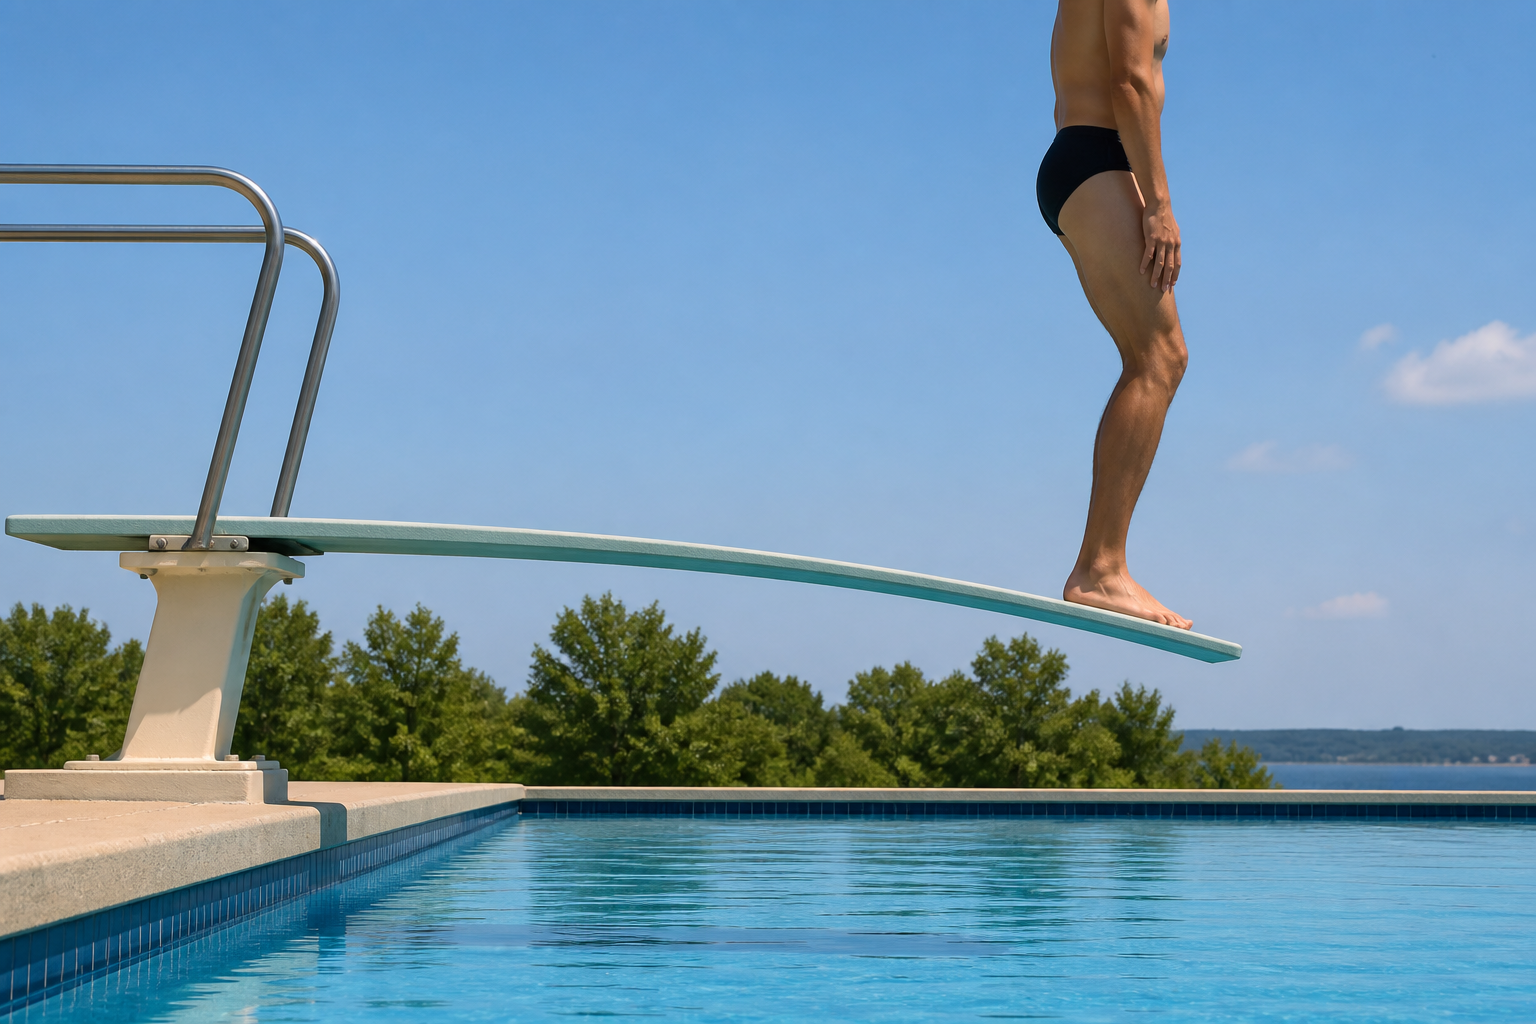
\includegraphics[width=0.58\linewidth]{images/book5/ai/b5-03-diving-board.png}

{\small Un plongeoir chargé~: contraintes et déformations réparties dans un milieu continu, courbé selon le profil cubique de la poutre encastrée --- et un ressort sur le point de restituer son \omterm{prop:b3:continuum-elasticity:energy}{énergie élastique}.}
\end{omfigure}

\section{Exercices}

\begin{exercise}[$\star$]\label{exo:b3:continuum-elasticity:1}
(a) Vérifier les unités~: qu'est-ce qu'un pascal en kg, m, s, et quelle
est l'unité de la déformation~? (b) Un câble d'acier travaille à $\sigma =
\qty{200}{MPa}$~: calculer sa déformation. (c) Un élastique ($E \approx
\qty{2}{MPa}$) est étiré au double de sa longueur~: quelle
«~déformation~» est-ce, et pourquoi le cadre de ce chapitre ne
s'applique-t-il pas vraiment~? (d) Classer par densité d'\omterm{prop:b3:continuum-elasticity:energy}{énergie
élastique} emmagasinée à leur contrainte de service~: l'acier à
\qty{200}{MPa}, le caoutchouc à \qty{1}{MPa}.
\end{exercise}

\begin{exercise}[$\star$]\label{exo:b3:continuum-elasticity:2}
Calculer le \omterm{def:b3:continuum-elasticity:strain}{tenseur des déformations} de chaque \omterm{def:b3:continuum-elasticity:strain}{champ de déplacement} et
décrire la distorsion~: (a) $\vect u = \alpha(x, y, z)$~; (b) $\vect u =
(\gamma y, 0, 0)$~; (c) $\vect u = (-\omega y, \omega x, 0)$~; (d)
$\vect u = (\varepsilon x, -\nu\varepsilon y, -\nu\varepsilon z)$ ---
quelle expérience le réalise~?
\end{exercise}

\begin{exercise}[$\star$]\label{exo:b3:continuum-elasticity:3}
La base d'une colonne de granite de hauteur $h$ supporte la contrainte $\sigma
= \rho gh$. (a) L'obtenir à partir de l'équation d'équilibre avec la
pesanteur. (b) Le granite s'écrase vers \qty{200}{MPa}~: quelle est la
colonne la plus haute~? (c) L'Everest fait \qty{8.8}{km}~: commenter.
(d) Pourquoi une montagne peut-elle être un peu plus haute qu'une
colonne de sa propre roche (penser à la forme)~?
\end{exercise}

\begin{exercise}[$\star$]\label{exo:b3:continuum-elasticity:4}
Une barre d'acier ($E = \qty{200}{GPa}$, $\nu = 0.30$) est étirée de
$\varepsilon = \num{e-3}$. (a) Déformation latérale~? (b) Variation
relative de volume~? (c) Pour quel $\nu$ le volume ne changerait-il pas
du tout, et quel matériau courant en est proche~? (d) Pourquoi
$\nu > 1/2$ est-il impossible (penser à une compression
hydrostatique)~?
\end{exercise}

\begin{exercise}[$\star\star$]\label{exo:b3:continuum-elasticity:5}
Contrainte circonférentielle. Un cylindre à paroi mince (rayon $R$, épaisseur $t \ll
R$) contient une pression $p$. (a) En équilibrant les forces sur un
demi-cylindre de longueur unité, montrer que la paroi porte la
contrainte tangentielle $\sigma_\theta = pR/t$. (b) Montrer que la
contrainte longitudinale (équilibre sur une section droite) vaut $pR/2t$~: un cylindre est deux fois plus
sollicité en circonférence qu'en longueur --- dans quel sens éclatent
les saucisses~? (c) Une bouteille de plongée~: $p =
\qty{200}{bar}$, $R = \qty{9}{cm}$, $t = \qty{5}{mm}$~: calculer
$\sigma_\theta$ et comparer à une limite d'élasticité de l'acier de
\qty{700}{MPa}. (d) Pourquoi les réservoirs haute pression ont-ils des
fonds hémisphériques~?
\end{exercise}

\begin{exercise}[$\star\star$]\label{exo:b3:continuum-elasticity:6}
Un bloc de caoutchouc ($E = \qty{3.0}{MPa}$, $\nu \approx 0.5$), de base $10
\times \qty{10}{cm}$ et de hauteur \qty{2}{cm}, est collé entre deux
plaques~; la plaque supérieure est poussée latéralement avec
\qty{150}{N}. (a) Calculer $G$. (b) Contrainte de cisaillement et angle
de cisaillement $\gamma = \sigma_{xy}/G$~; déplacement latéral de la
plaque supérieure. (c) Pourquoi $\nu \approx 1/2$ pour le caoutchouc
(qu'est-ce qui est difficile et qu'est-ce qui est facile pour un
enchevêtrement de chaînes polymères)~? (d) De tels blocs de caoutchouc
portent des immeubles entiers en zone sismique~: quelle propriété de
cet appui protège le bâtiment, la rigidité en compression ou la
souplesse en cisaillement~?
\end{exercise}

\begin{exercise}[$\star\star$]\label{exo:b3:continuum-elasticity:7}
Une corde d'escalade, de longueur $L = \qty{20}{m}$, de section $S =
\qty{80}{mm^2}$, de module effectif $E = \qty{1.2}{GPa}$. (a) Sa
raideur $k = ES/L$. (b) Un grimpeur de \qty{80}{kg} chute librement de
\qty{4}{m} avant que la corde n'agisse~: en égalant les énergies,
trouver l'allongement maximal de la corde (résoudre l'équation du
second degré~; négliger en première approche la chute poursuivie
pendant le freinage). (c) En déduire la force maximale et la
décélération maximale en $g$. (d) Pourquoi une corde ayant retenu une
chute dure doit-elle être réformée (où est passée l'énergie, et que dit
la courbe contrainte--déformation)~?
\end{exercise}

\begin{exercise}[$\star\star$]\label{exo:b3:continuum-elasticity:8}
Torsion. Un fil de rayon $a$, de longueur $L$ et de module de
cisaillement $G$ est tordu d'un angle $\theta$. (a) Montrer qu'un tube
de rayon $r$ à l'intérieur subit l'angle de cisaillement
$\gamma(r) = r\theta/L$. (b) Sa contrainte de cisaillement vaut
$G\gamma$~: intégrer $r \times$ contrainte sur la section pour obtenir
le couple de rappel $\Gamma = (\pi Ga^4/2L)\,\theta$. (c) Le $a^4$~:
diviser le rayon par deux, et de quel facteur chute la rigidité de
torsion~? (d) Cette extrême souplesse explique que Cavendish (1798) ait
suspendu sa balance à un fil très fin~: pour $a = \qty{25}{\micro m}$, $L =
\qty{1}{m}$, $G = \qty{40}{GPa}$, calculer $C = \pi Ga^4/2L$ et la
période avec un fléau de moment d'inertie $I = \qty{5e-4}{kg.m^2}$.
\end{exercise}

\begin{exercise}[$\star\star$]\label{exo:b3:continuum-elasticity:9}
(a) À partir de la démonstration en onde plane de
\cref{prop:b3:continuum-elasticity:waves}, calculer $c_{\text{P}}$ et
$c_{\text{S}}$ pour l'acier ($E = \qty{200}{GPa}$, $\nu = 0.29$, $\rho =
\qty{7.85e3}{kg/m^3}$). (b) Comparer $c_{\text{P}}$ à la vitesse dans
un barreau mince $\sqrt{E/\rho}$ et expliquer l'écart en une phrase.
(c) Pour l'eau ($\mu = 0$, module de compressibilité \qty{2.2}{GPa})~:
la vitesse S et la vitesse P. (d) De quel angle le mouvement de la
matière dans une \omterm{prop:b3:continuum-elasticity:waves}{onde P} diffère-t-il de celui d'une \omterm{prop:b3:continuum-elasticity:waves}{onde S}, et comment
un sismomètre à trois composantes les distingue-t-il~?
\end{exercise}

\begin{exercise}[$\star\star\star$]\label{exo:b3:continuum-elasticity:10}
Flexion. Une poutre est courbée à un rayon de courbure $R$~; ses fibres
intérieures raccourcissent, ses fibres extérieures s'allongent, et une
\emph{surface neutre} intermédiaire garde sa longueur. (a) Montrer que
la fibre située à la distance $y$ de la surface neutre a la déformation
$\varepsilon = y/R$, donc la contrainte $Ey/R$. (b) En sommant les
moments sur la section, montrer que le moment fléchissant vaut
$M = EI/R$ avec $I = \int y^2\,\dd S$ (le \emph{moment quadratique})~;
calculer $I$ pour un rectangle de largeur $b$ et de hauteur $h$. (c) Le
$h^3$~: pourquoi une planche fléchie à plat s'affaisse-t-elle
visiblement alors que la même planche de chant paraît rigide~?
Calculer le rapport pour $b/h = 5$. (d) Pour une poutre encastrée de
longueur $L$ chargée par $F$ à son extrémité, la flèche vaut
$\delta = FL^3/3EI$ (admis)~: estimer $\delta$ pour un plongeoir
($L = \qty{1.8}{m}$, $b = \qty{50}{cm}$, $h = \qty{3.5}{cm}$, bois $E
= \qty{12}{GPa}$) sous un plongeur de \qty{75}{kg}, et commenter.
\end{exercise}

\begin{exercise}[$\star\star\star$]\label{exo:b3:continuum-elasticity:11}
Flambage. Une colonne élancée (longueur $L$, rigidité de flexion $EI$),
articulée à ses deux extrémités, porte une charge axiale $P$. Supposons
qu'elle s'incurve latéralement de $y(x)$. (a) Montrer que la charge
exerce alors le moment fléchissant $M(x) = -Py(x)$ autour de l'axe
déplacé, donc $EI\,y'' = -Py$. (b) Avec $y(0) = y(L) = 0$, montrer
qu'une flèche non nulle devient possible pour la première fois à la
charge critique d'Euler $P_{\text{c}} = \pi^2EI/L^2$. (c) Calculer
$P_{\text{c}}$ pour un mètre de menuisier ($b = \qty{3}{cm}$, $h = \qty{1.5}{mm}$, $E = \qty{12}{GPa}$) et
comparer à la poussée de votre main. (d) Expliquer à partir de $I$
pourquoi les os, le bambou et les cadres de bicyclette sont des
\emph{tubes}.
\end{exercise}

\begin{exercise}[$\star\star\star$]\label{exo:b3:continuum-elasticity:12}
La vitesse du son dans un solide, à partir des atomes. Modélisons un
solide par des chaînes d'atomes de pas $a$, reliés par des «~ressorts~»
de raideur $\kappa$~; masse atomique $m$. (a) Montrer que l'étirement
de la chaîne se ramène à la traction du milieu continu avec $E = \kappa/a$ (compter les ressorts
par unité d'aire, l'allongement par ressort). (b) Montrer que
$\rho = m/a^3$ et conclure que $c =
\sqrt{E/\rho} = a\sqrt{\kappa/m}$. (c) Estimer $\kappa$ à partir de la
profondeur d'une liaison interatomique ($\sim\qty{3}{eV}$ sur $\sim
\qty{0.1}{nm}$)~: $\kappa \sim \qty{50}{N/m}$~; avec $a =
\qty{2.5e-10}{m}$ et $m = \qty{1e-25}{kg}$, estimer $c$. (d) Comparer
aux vitesses du son mesurées dans les métaux, et conclure de quoi est
faite l'élasticité de tous les jours.
\end{exercise}

\section{Problème~: écouter la Terre}

\begin{problem}[{Problème du week-end --- comment les séismes ont
révélé le noyau liquide}]\label{pb:b3:continuum-elasticity:1}
Un seul séisme fait sonner la planète entière, et les deux \omterm{prop:b3:continuum-elasticity:waves}{ondes
élastiques} de ce chapitre, en la traversant, la radiographient. Ce
problème suit la physique depuis la \omterm{thm:b3:continuum-elasticity:hooke}{loi de Hooke} dans le granite
jusqu'à la découverte, par Oldham en 1906, que la Terre a un noyau ---
avec l'estimation de sa taille en rayons rectilignes. On prend pour la
roche de la croûte et du manteau $E = \qty{75}{GPa}$, $\nu = 1/4$,
$\rho = \qty{2.7e3}{kg/m^3}$~; rayon terrestre $R_{\text{E}} =
\qty{6371}{km}$.

\medskip\noindent\textbf{Partie I --- La roche, solide élastique.}
\begin{enumerate}
  \item Calculer les coefficients de Lamé $\mu$ et $\lambda$ de cette
        roche, et observer que $\nu = 1/4$ les rend égaux.
  \item Calculer $c_{\text{P}}$ et $c_{\text{S}}$, et vérifier que
        $c_{\text{P}} = \sqrt3\,c_{\text{S}}$.
  \item Un séisme fait glisser deux faces rocheuses de plusieurs mètres
        en quelques secondes~: estimer la déformation relâchée si un
        glissement de \qty{2}{m} détend la roche sur une échelle de
        \qty{50}{km}, ainsi que la contrainte accumulée.
  \item À partir de la densité d'énergie $w = \tfrac12 E\varepsilon^2$,
        estimer l'\omterm{prop:b3:continuum-elasticity:energy}{énergie élastique} par mètre cube, puis l'énergie
        contenue dans un volume de $50 \times 50 \times \qty{20}{km^3}$~;
        comparer à une mégatonne (\qty{4.2e15}{J}).
  \item Pourquoi l'\omterm{prop:b3:continuum-elasticity:waves}{onde S} secoue-t-elle en général les bâtiments plus
        fort que l'\omterm{prop:b3:continuum-elasticity:waves}{onde P} (penser à la direction du mouvement du sol
        pour une onde qui arrive d'en bas)~?
  \item Dans laquelle des deux ondes le sol change-t-il de volume~?
\end{enumerate}

\medskip\noindent\textbf{Partie II --- Les deux arrivées du sismomètre.}
\begin{enumerate}[resume]
  \item Une station enregistre l'arrivée P, puis l'arrivée S $\Delta t$
        plus tard. Pour une source à la distance $d$ (assez courte
        pour des rayons rectilignes), montrer que
        \[
        d = \frac{\Delta t}{\dfrac{1}{c_{\text{S}}} -
        \dfrac{1}{c_{\text{P}}}} .
        \]
  \item Évaluer le coefficient~: combien de kilomètres par seconde de
        retard S--P~?
  \item Une station mesure $\Delta t = \qty{28}{s}$~: à quelle
        distance est le séisme~?
  \item Une station donne une distance, non un lieu~: combien de
        stations déterminent l'épicentre, et comment, géométriquement~?
  \item Les sirènes d'alerte japonaises retentissent quelques secondes
        avant la forte secousse~: pour un séisme à \qty{80}{km} sous
        une ville, quel préavis le retard P--S fournit-il à lui seul~?
  \item Les alertes modernes ajoutent la vitesse de la lumière~:
        l'\omterm{prop:b3:continuum-elasticity:waves}{onde P} détectée près de la source est annoncée par radio en
        avance sur les deux ondes. Pour une ville à \qty{200}{km} de
        l'épicentre, combien de temps après la rupture l'\omterm{prop:b3:continuum-elasticity:waves}{onde S}
        arrive-t-elle, et quel préavis peut donner un message radio
        émis à la première arrivée P, à \qty{20}{km} de la source~?
\end{enumerate}

\medskip\noindent\textbf{Partie III --- Des ondes qui traversent la planète.}
\begin{enumerate}[resume]
  \item Aux pressions du manteau profond, les modules croissent~: les
        vitesses P atteignent \qty{13.7}{km/s} à la base du manteau.
        En prenant une moyenne grossière $c_{\text{P}} \approx \qty{10}{km/s}$, combien de temps
        une \omterm{prop:b3:continuum-elasticity:waves}{onde P} met-elle à traverser la Terre en diamètre~?
  \item Des stations enregistrent des séismes venus de l'autre côté du
        globe~: que dit la seule existence de ces arrivées sur la Terre
        profonde (est-elle élastique~? fondue de part en part~?)~?
  \item Définir l'angle épicentral $\Delta$ (angle au centre de la
        Terre entre la source et la station). Pour des rayons
        rectilignes, montrer que la corde vaut
        $2R_{\text{E}}\sin(\Delta/2)$.
  \item Évaluer la corde et son temps de trajet rectiligne pour
        $\Delta = 60^\circ$ à la moyenne $c_{\text{P}} \approx
        \qty{10}{km/s}$.
  \item Vers 1900, Oldham remarqua que les \omterm{prop:b3:continuum-elasticity:waves}{ondes S} sont enregistrées
        jusqu'à $\Delta \approx 103^\circ$ puis \emph{disparaissent}~:
        plus de S directe au-delà. Quelle propriété d'une région
        profonde de la Terre tue les \omterm{prop:b3:continuum-elasticity:waves}{ondes S}, et quel état de la
        matière possède cette propriété~?
  \item Au-delà de $103^\circ$ les \omterm{prop:b3:continuum-elasticity:waves}{ondes P} ne sont pas absentes mais
        affaiblies, retardées et déplacées (une «~zone d'ombre~»
        jusqu'à $\approx 142^\circ$)~: pourquoi une région liquide
        retarde-t-elle et réfracte-t-elle les \omterm{prop:b3:continuum-elasticity:waves}{ondes P} sans les
        arrêter~?
  \item Conclure en une phrase sur ce qui siège au centre de la Terre.
\end{enumerate}

\medskip\noindent\textbf{Partie IV --- Peser le noyau avec une règle.}
\begin{enumerate}[resume]
  \item Un rayon S rectiligne partant de la source rase le noyau si sa
        distance minimale au centre égale le rayon du noyau
        $R_{\text{c}}$. Montrer que ce rayon rasant atteint la surface
        à l'angle épicentral $\Delta^* =
        2\arccos(R_{\text{c}}/R_{\text{E}})$.
  \item À partir de $\Delta^* = 103^\circ$, calculer $R_{\text{c}}$.
  \item La valeur moderne est \qty{3480}{km}~: calculer votre erreur et
        en expliquer le \emph{signe} --- les vrais rayons se recourbent
        vers la surface à mesure que la vitesse croît avec la
        profondeur~; dites si les rayons rectilignes surestiment ou
        sous-estiment le noyau.
  \item En 1936 Inge Lehmann trouva de faibles arrivées P
        \emph{à l'intérieur} de la zone d'ombre~: qu'en a-t-elle
        conclu sur ce qui siège au sein du noyau liquide~?
  \item La graine a un rayon de \qty{1220}{km} et elle est solide~:
        proposer l'observation ondulatoire qui pourrait confirmer cette
        solidité (quelle onde y existe-t-il que le noyau externe
        interdit~?).
  \item Résumer le résultat nommé~: deux vitesses d'\omterm{prop:b3:continuum-elasticity:waves}{ondes élastiques}
        dans la roche ($5.8$ et \qty{3.3}{km/s}), une onde manquante
        au-delà de $103^\circ$ et une règle donnent un noyau liquide de
        rayon $\approx \qty{4000}{km}$ --- à $15\%$ près de la valeur
        moderne \qty{3480}{km}, mesurée à travers \qty{6000}{km} de
        roche solide.
\end{enumerate}
\end{problem}
